\input header.tex

\begin{document}
\title{PFN インターン選考課題 2019 バックエンド分野}
\author{福岡 拓也}
\date{}
\maketitle

\small


\section*{実行環境}
\begin{itemize}
    \item macOS Mojave (10.14.4)
    \item Python 3.7.1
        \begin{itemize}
            \item Flask 1.0.2
        \end{itemize}
    \item Apple LLVM version 10.0.1 (clang-1001.0.46.4)
\end{itemize}

\section*{問題1.1 (サーバーの作成)}
サーバープログラムの開発には, Pythonの軽量フレームワークFlaskを用いた. 
環境変数DATA\_DIRでジョブの存在するディレクトリを指定することができる. 
Created (作成日時)はタイムスタンプではなく秒に直したものを, 
Priority (優先度) については, Highの場合は1を, Lowの場合は0を返すような仕様とした. 
また, 同じ時刻に対して複数のジョブを返すことが可能である.

\begin{lstlisting}[]
$ cd server
$ DATA_DIR=../test/data_test1 FLASK_APP=server.py flask run &
$ curl http://localhost:5000/jobs/00:00:03

{"Jobs":[{"Created":3,"JobID":2,"Priority":1,"Tasks":[3,5]}]}
\end{lstlisting}

サーバーについてのユニットテストは以下のコマンドで走らせることができる.

\begin{lstlisting}[]
$ cd server
$ DATA_DIR=./data FLASK_APP=server.py flask run &
$ python test.py
\end{lstlisting}

\section*{問題1.2 (ワーカーの作成)}

%通信で取得したJsonをパースするライブラリとしてJson11を使用した。
ワーカーは以下のコマンドで走らせることができる.
標準出力には時刻とExecuting Pointを、エラー出力にはジョブが終了した時にそのジョブの優先度と、待ち時間 (終了時間 - 開始時間 - タスクの総量) を出力する.

\begin{lstlisting}[]
$ cd server
$ FLASK_APP=server.py flask run &
$ cd ../worker
$ make
$ MAXTIME=4000 CAPACITY=-1 PRIORITY_RANGE=1 ./worker 1>../plot/log1_2 2>../plot/wait1_2
\end{lstlisting}

サーバーとワーカーについての統合テストは以下のように走らせることができる.
統合テスト内でサーバーの起動と終了を行なっているので、予めサーバーを起動させる必要はない.

\begin{lstlisting}[]
$ cd test
$ ./test_run.sh
\end{lstlisting}

\begin{figure}[htbp]
  \centering
  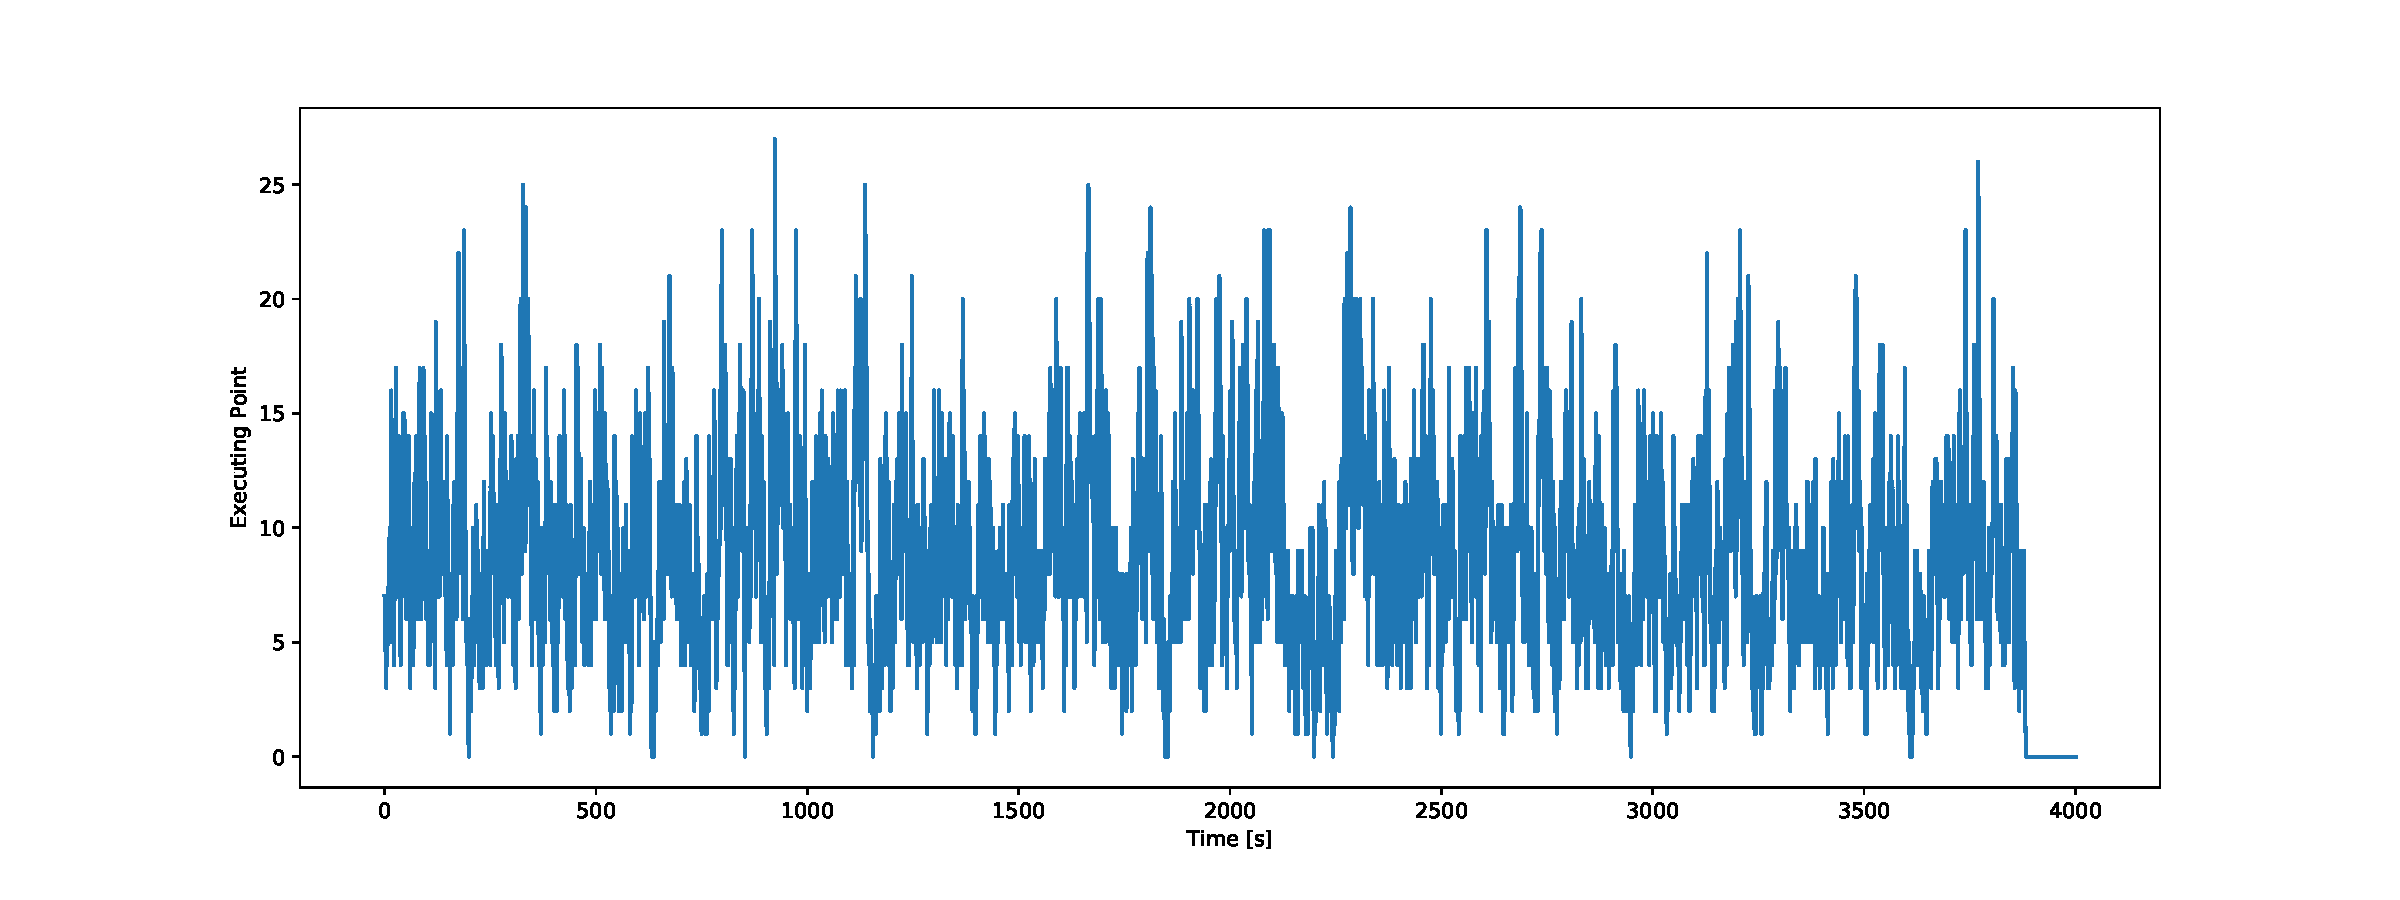
\includegraphics[width=\linewidth]{imgs/log1_2.pdf}
  \caption{The transition of Executing Point with no capacity and no priority (1-2)}
  \label{fig:log1_2}
\end{figure}

\clearpage
\section*{問題2.1 (キャパシティの追加)}

実行していないジョブと実行されているジョブをそれぞれ別のリストで管理し、実行時に移動させるような設計となっている.

\begin{lstlisting}[]
$ cd server
$ FLASK_APP=server.py flask run &
$ cd ../worker
$ make
$ MAXTIME=4000 CAPACITY=15 PRIORITY_RANGE=1 NAIVE=1 ./worker 1>../plot/log2_1 2>../plot/wait2_1
\end{lstlisting}

\begin{figure}[htbp]
  \centering
  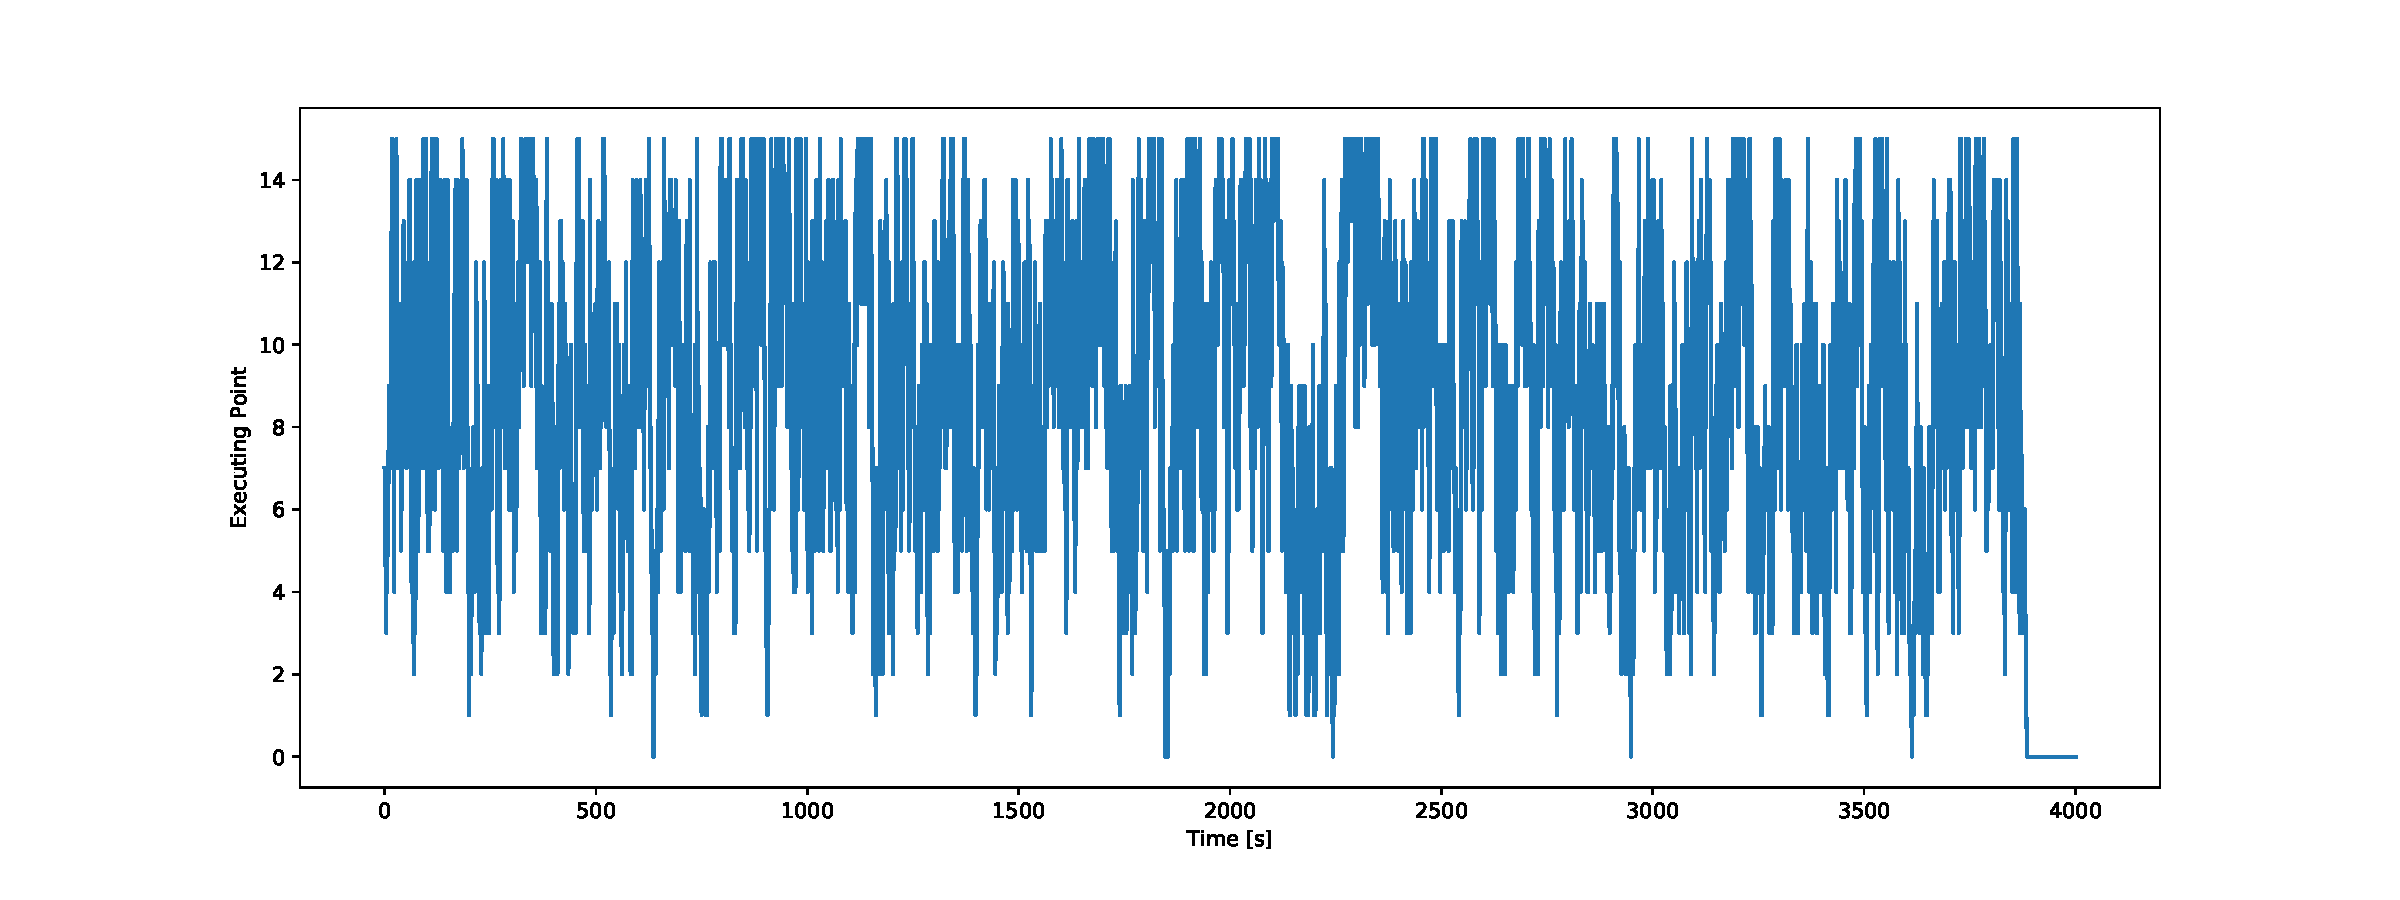
\includegraphics[width=\linewidth]{imgs/log2_1.pdf}
  \caption{The transition of Executing Point with no priority (2-1)}
  \label{fig:log2_1}
\end{figure}

\section*{問題2.2 (優先度の追加)}

さらに, 優先度毎に別のリストでジョブを管理するようにした.
また, 高い優先度のジョブの実行の妨げが生じないように, 実行を待っている高い優先度のジョブが存在する時には, 低い優先度のジョブの実行を一切行わない設計にしている.
例えば、Executing Pointの余裕が5であり, 低い優先度のジョブの次に実行されるタスクの大きさが3で, 高い優先度のジョブの次に実行されるタスクの大きさが6の場合, 低い優先度のジョブの実行は見送ることになる.
実行時には問題2.3の実装と区別するために, 環境変数NAIVE=1を設定する.

\begin{lstlisting}[]
$ cd server
$ FLASK_APP=server.py flask run &
$ cd ../worker
$ make
$ MAXTIME=4000 CAPACITY=15 PRIORITY_RANGE=2 NAIVE=1 ./worker 1>../plot/log2_2 2>../plot/wait2_2
\end{lstlisting}

\begin{figure}[htbp]
  \centering
  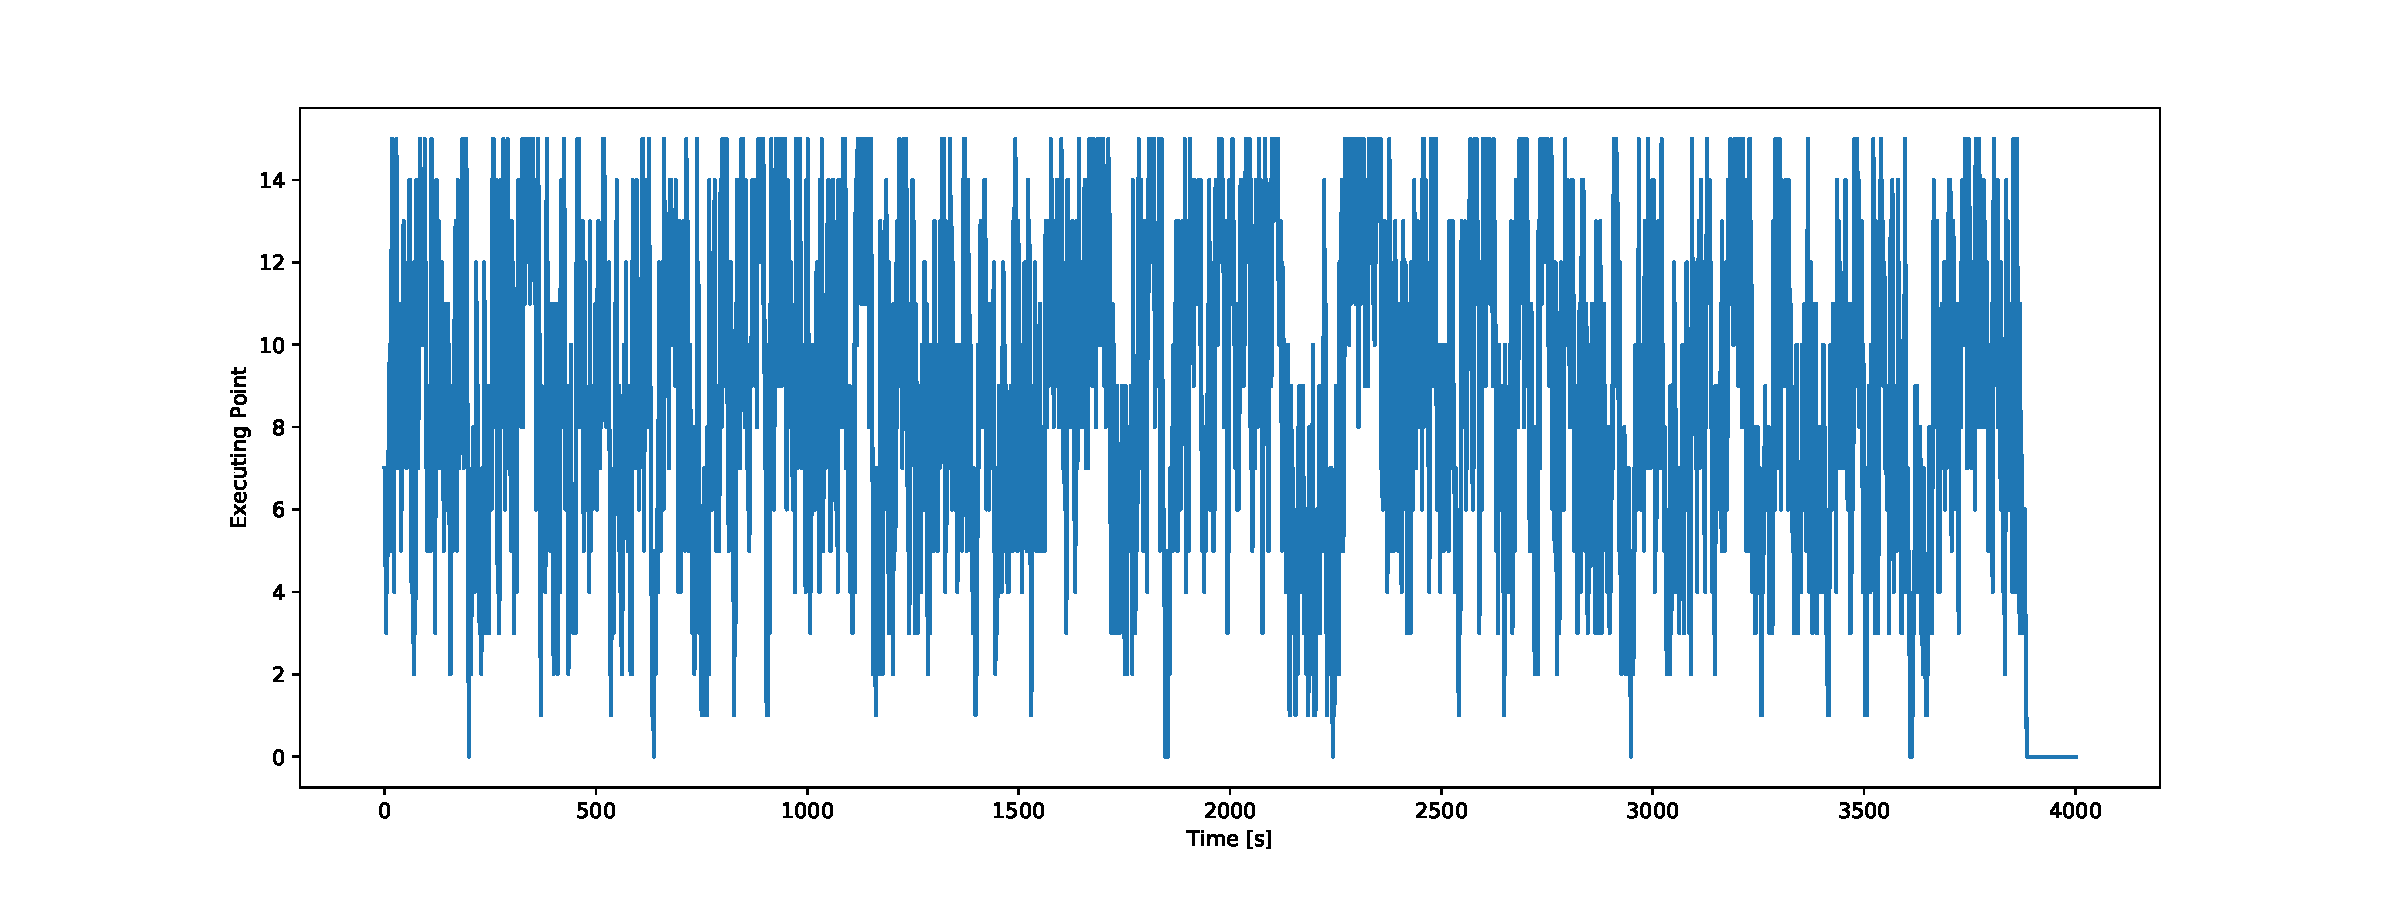
\includegraphics[width=\linewidth]{imgs/log2_2.pdf}
  \caption{The transition of Executing Point with the naive scheduling (2-2)}
  \label{fig:log2_2}
\end{figure}

\clearpage
\section*{問題2.3 (実行スケジューリングの効率化)}

\begin{lstlisting}[]
$ cd server
$ FLASK_APP=server.py flask run &
$ cd ../worker
$ make
$ MAXTIME=4000 CAPACITY=15 PRIORITY_RANGE=2 ./worker 1>../plot/log4 2>../plot/wait2_3
\end{lstlisting}

\begin{figure}[htbp]
  \centering
  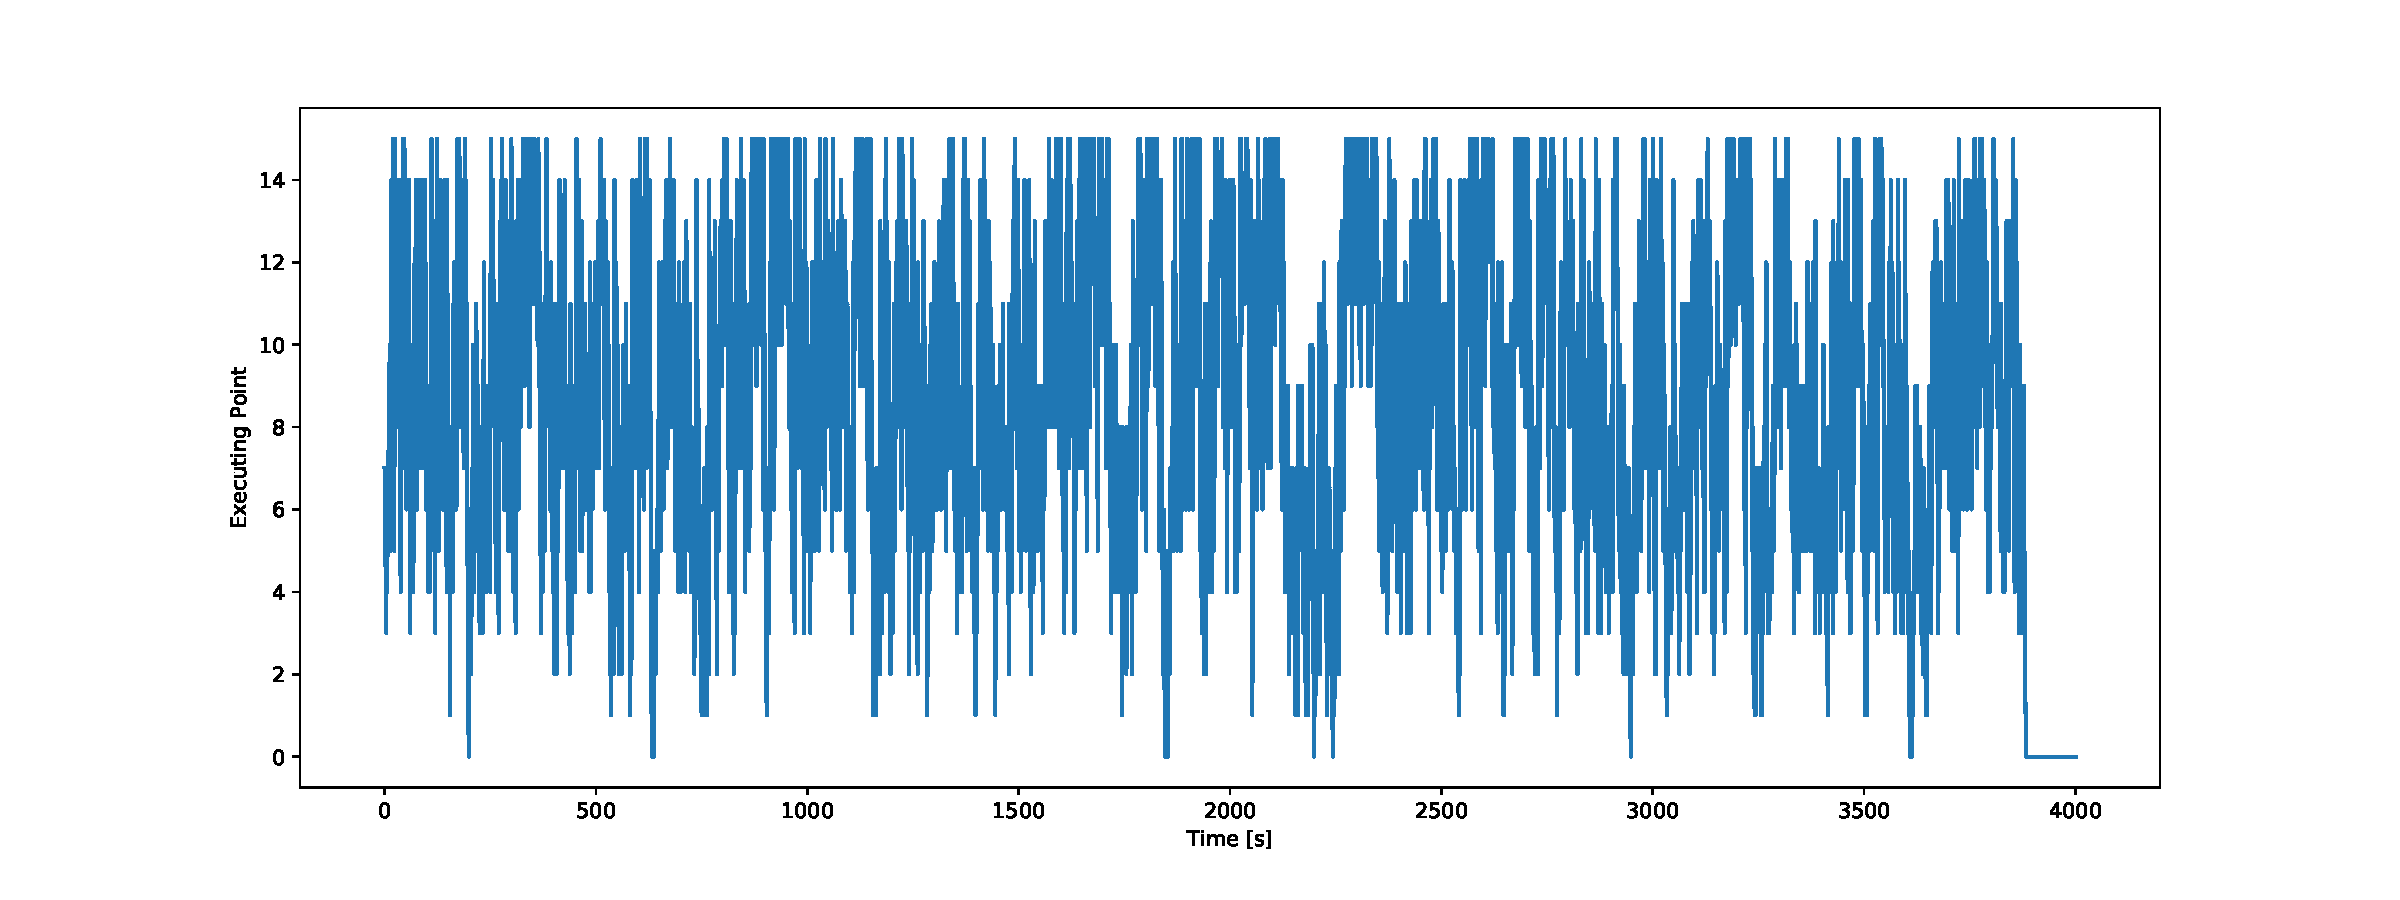
\includegraphics[width=\linewidth]{imgs/log2_3.pdf}
  \caption{The transition of Executing Point with the efficient scheduling (2-3)}
  \label{fig:log2_3}
\end{figure}

問題2.2のジョブのスケジューリングについて, 高い優先度のジョブが存在する時に無条件で低い優先度のジョブの実行を見送るのは効率が悪い. 
したがって, ジョブのスケジューリングの先読みを行い, 近い将来行われる高い優先度のジョブの実行に妨げのない場合にのみ限り低い優先度のジョブの実行を許可するようにする. 先読みの秒数は長い方がより正確に予測ができるが計算量が大きくなるという欠点がある. そのトレードオフを考えて, 今回はキャパシティの大きさと同じだけの秒数だけの先読みを行うことにする. そうすることで, 少なくとも直近の高い優先度のジョブについては, 低い優先度のジョブの実行に妨げられず実行ができることが保証できる. 以下具体例を用いて説明する. 

まず, 現在実行されているジョブの影響のみを考えた, Executing Pointの余裕分 (以下Spare Pointと呼ぶ) の推移を計算する. キャパシティが8で, 2と4の大きさのタスクが実行されていたとすると, Spare Pointは

2, 4, 6, 7, 8, 8, 8, 8, 8

\noindent と推移する. また, この時優先度の高いタスクの大きさが5のジョブが実行を待っているとすると, このジョブは最短で2秒後に実行することができるとわかり, このジョブが実際2秒後に実行されるとすると, この時のSpare Pointの推移は

2, 4, 1, 3, 5, 6, 7, 8, 8

\noindent と予測できる. 同様に, 優先度の高い次のジョブのタスクの大きさが3であった場合には, このジョブは3秒後に実行することができて, このジョブの実行を予約した時のSpare Pointの推移は

2, 4, 1, 0, 3, 5, 7, 8, 8

\noindent となる. これを待機している優先度の高いジョブについて全て適応して, その後に初めて, それでも実行できる優先度の低いジョブを実行する.
補足であるが, 現在のSpare Pointが0になった時点で探索を終了して次の時刻に進むようにすることで, 計算量を削減している.

待ち時間を、ジョブ終了時刻 - ジョブ生成時刻 - タスクの総量と定義して, 改善前と改善後の待ち時間をヒストグラムで比較したのが次のグラフである. 
待ち時間の平均は, 改善前の実装については高い優先度と低い優先度のジョブそれぞれについて, 1.88と0.208であるのに対して, 
改善後については0.81と0.0755であり, 2倍以上待ち時間が改善されていることがわかる. 

\begin{figure}[htbp]
  \begin{minipage}[b]{0.40\hsize}
      \centering
      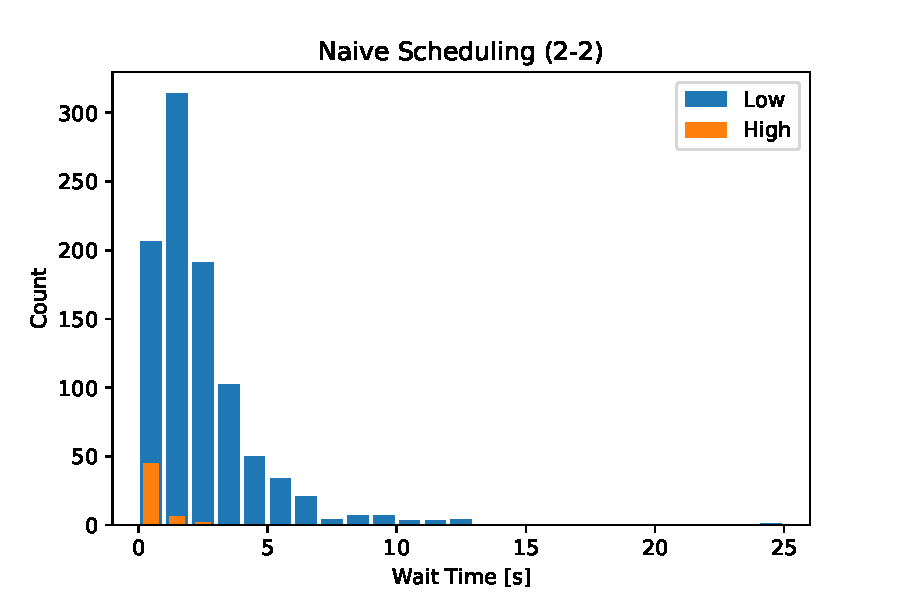
\includegraphics[width=8cm]{imgs/wait2_2.pdf}
      \caption{Count of waiting time in the naive implementation (2-2)}
      \label{fig:wait2_2}
  \end{minipage}
  \begin{minipage}{0.1\hsize}
    \hspace{0.05\hsize}
  \end{minipage}
  \begin{minipage}[b]{0.40\hsize}
      \centering
      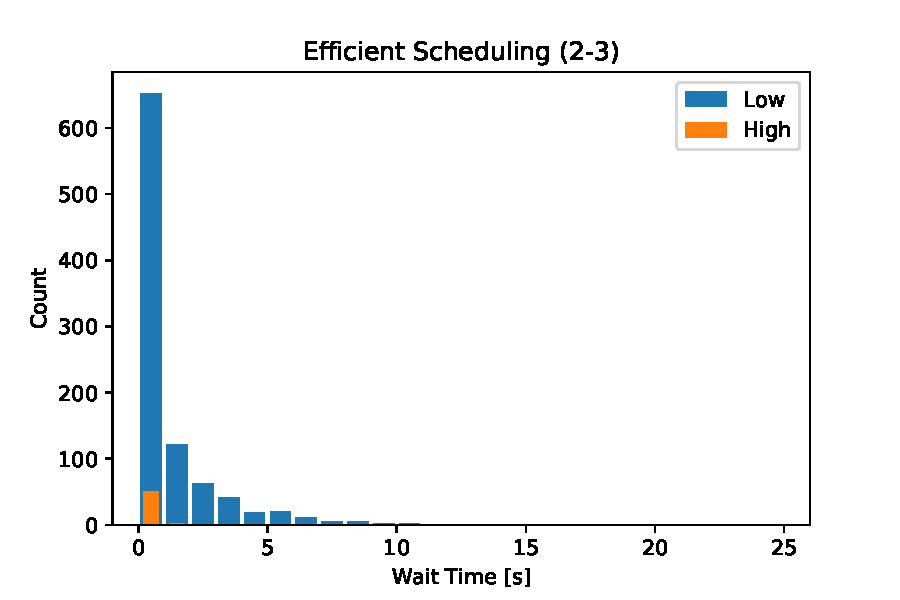
\includegraphics[width=8cm]{imgs/wait2_3.pdf}
      \caption{Count of waiting time in the efficient implementation (2-3)}
      \label{fig:wait2_3}
  \end{minipage}
\end{figure}

\clearpage
\section*{問題3.1 (0-100までの優先度に対応)}

\begin{lstlisting}[]
$ cd server
$ DATA_DIR=./data_num_priority NUM_PRIORITY=1 FLASK_APP=server.py flask run &
$ cd ../worker
$ make
$ MAXTIME=4000 CAPACITY=15 PRIORITY_RANGE=101 ./worker 1>../plot/log3_1 2>../plot/wait3_1
\end{lstlisting}

問題2-3のアルゴリズムに関しては, 優先度の個数が増えた場合でも同様に適用することができる.
問題2-1から問題2-2の拡張と同じように, 優先度の個数だけジョブを管理するリストを用意すれば, それがそのまま問題3-1の実装となる.
待ち時間の全平均は0.819である.

\begin{figure}[htbp]
  \centering
  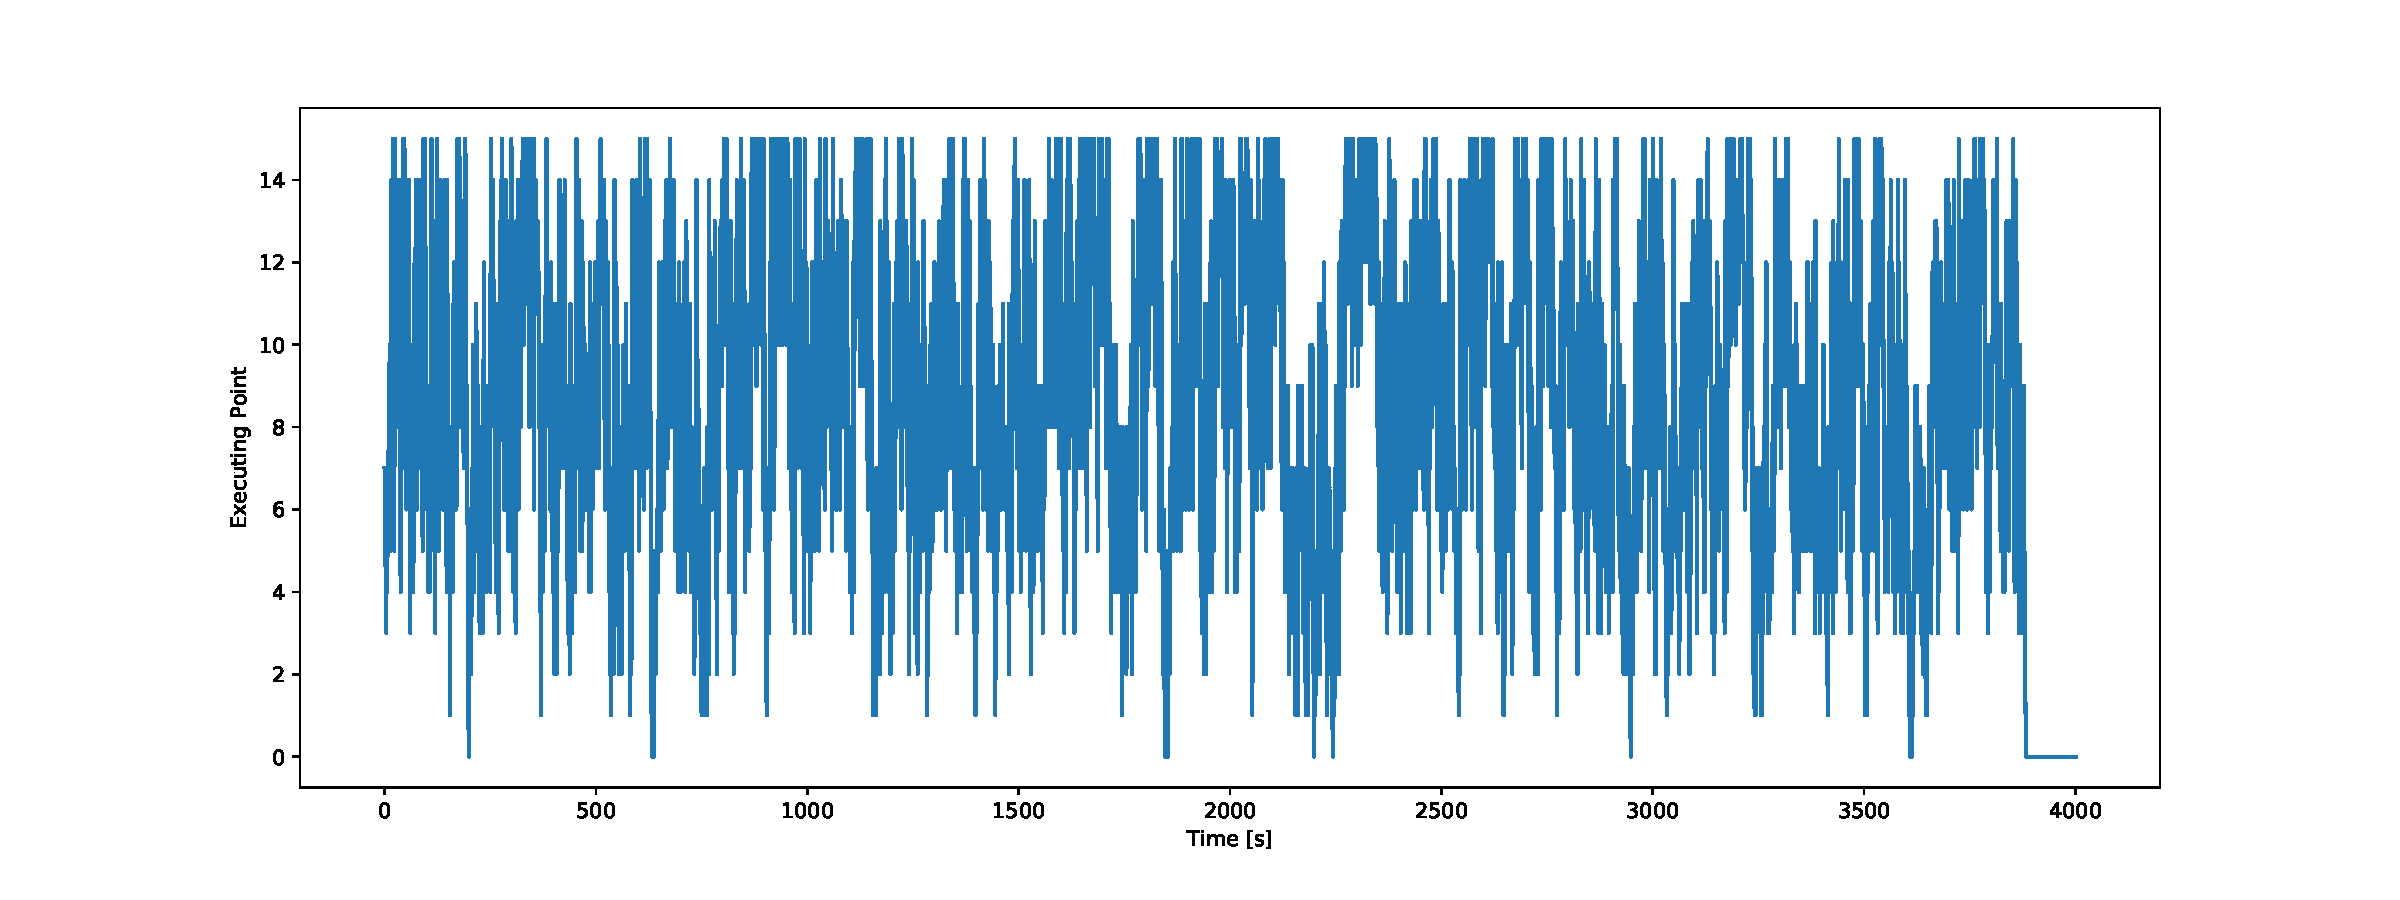
\includegraphics[width=\linewidth]{imgs/log3_1.pdf}
  \caption{The transition of Executing Point with the efficient scheduling (3-1)}
  \label{fig:log3-1}
\end{figure}


\begin{figure}[htbp]
  \centering
  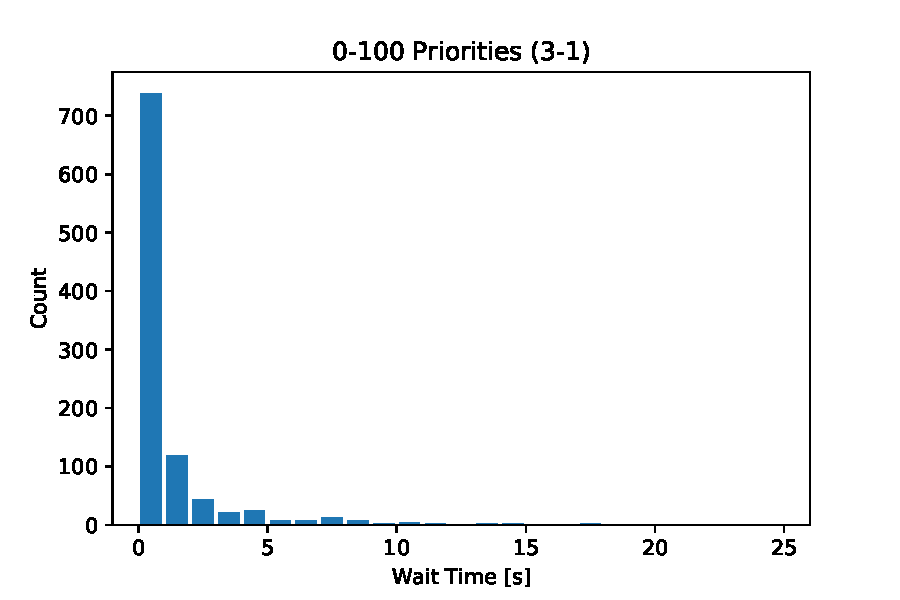
\includegraphics[width=8cm]{imgs/wait3_1.pdf}
  \caption{Count of waiting time in 0-100 priorities (3-1)}
  \label{fig:wait3-1}
\end{figure}

\end{document}
